% LuaLaTeX
\pdfvariable minorversion=7
\documentclass[10pt]{article}

% Packages
\usepackage[no-math]{fontspec}
\usepackage{geometry}
\usepackage{hyperref}
\usepackage[backend=biber]{biblatex} % we use the biber implementation of biblatex for bibliographies
\usepackage[nonumberlist, toc]{glossaries}
\usepackage{graphicx}
\usepackage{pdfpages}
\usepackage{booktabs}
\usepackage{float}
\usepackage{subcaption}
\usepackage{fancyhdr}
\usepackage{amsmath}
\usepackage{siunitx}

% Formatting
\geometry{letterpaper, portrait, margin=.85in}
\defaultfontfeatures{Ligatures=TeX}
\setmainfont[
    BoldFont       = Avenir Medium,
    ItalicFont     = Avenir Book Oblique,
    BoldItalicFont = Avenir Medium Oblique
]{Avenir Book}
\setmonofont{Andale Mono}
\sisetup{detect-all} % used by siunitx to always typeset units in the font of the current environment
\urlstyle{same}

\newcommand\theteamname{Midnight Sun Solar Car Team} % should not change normally
\newcommand\theuniversityname{University of Waterloo} % should also not change normally
\newcommand\theteamwebsite{www.uwmidsun.com} % should also not normally change
\newcommand\theteamphone{(519) 888-4567 x32978} % should also not normally change

\newcommand\thetitle{Preliminary Vehicle Design Report} % <--------------- add the title
\newcommand\thesubtitle{Electrical} % <--------------- add a subtitle or leave the field empty
\newcommand\theauthor{Minghao Ji} % <--------------- add an author with contact info or comment this line
\newcommand\theauthorcontact{minghao.ji@uwmidsun.com} % <--------------- add author's email or leave the field empty
\newcommand\thedate{October 15, 2017} % <--------------- update the date, use this format

\pagestyle{fancy}
\renewcommand{\headrulewidth}{0pt}
\lhead{\thetitle}
\rhead{\theteamname}

\begin{document}
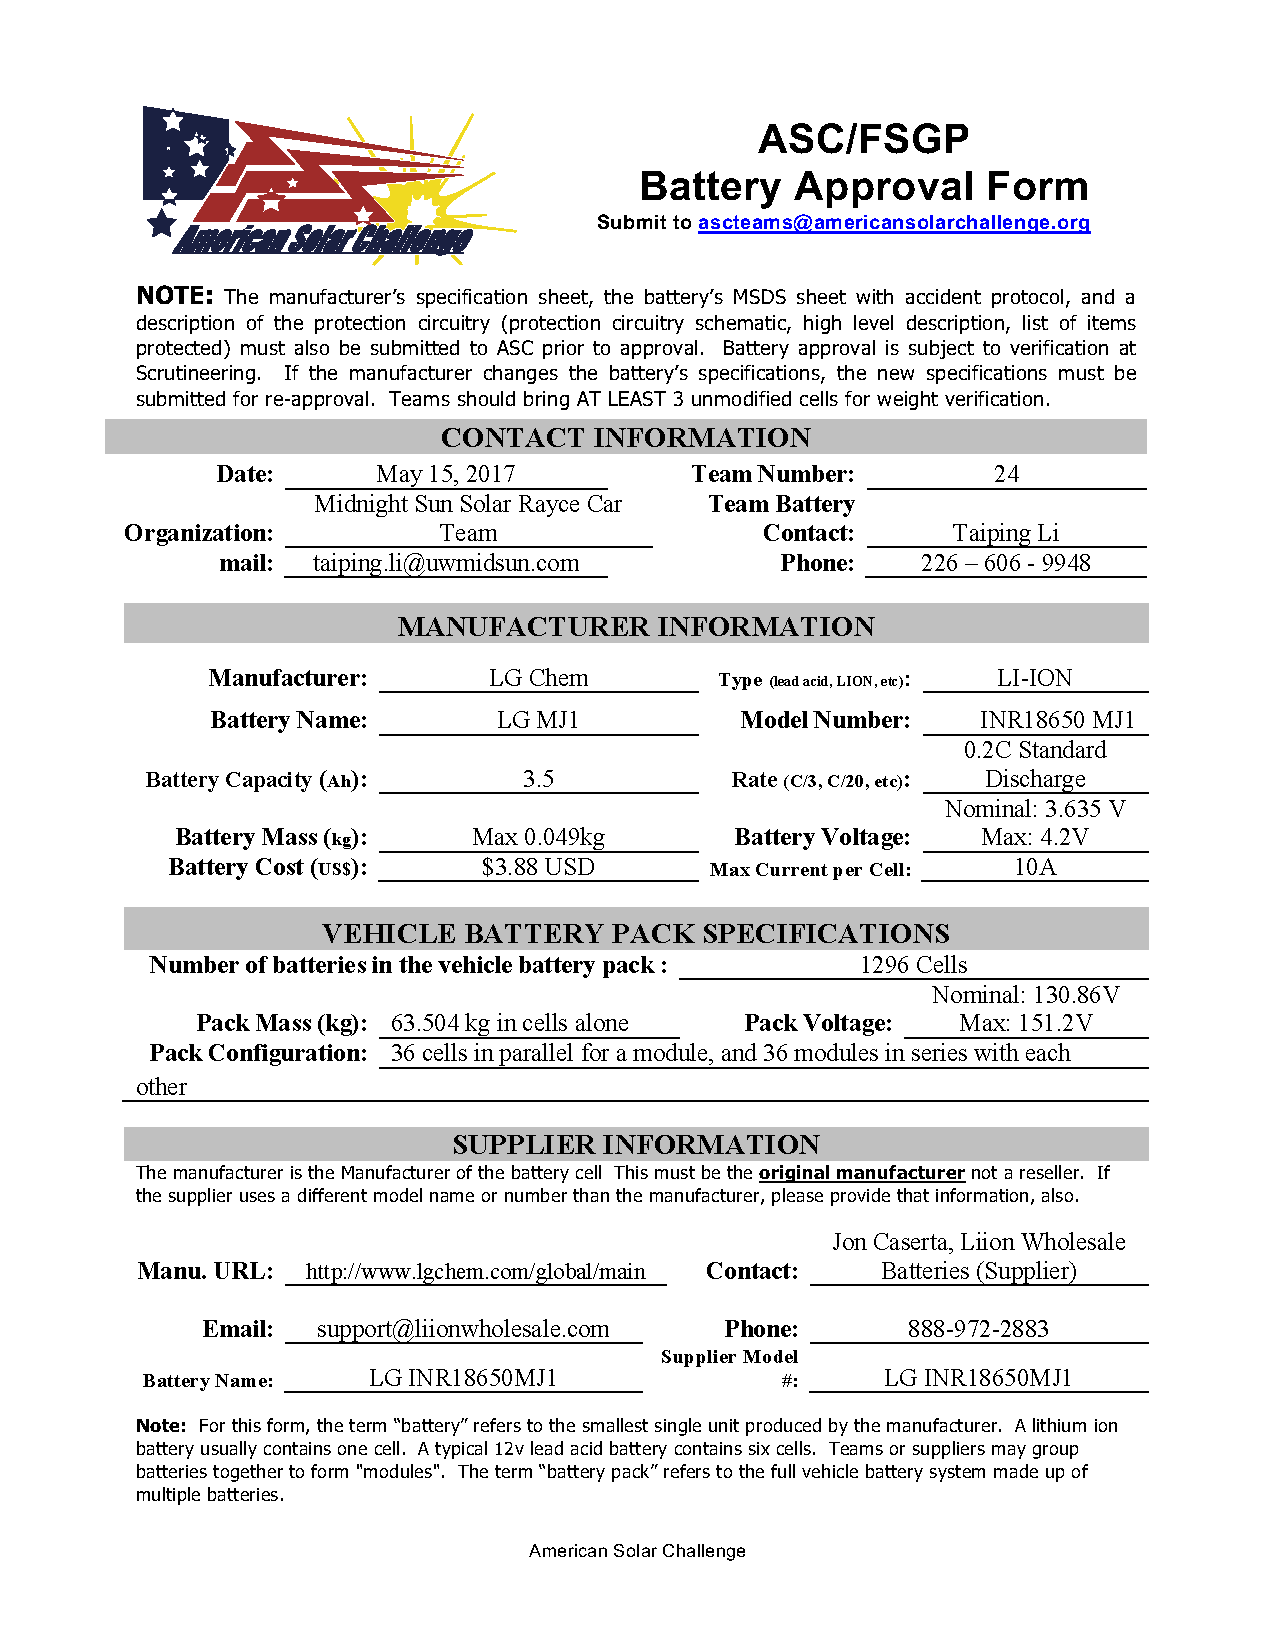
\includepdf[pages={-}]{forms/battery_approval_form.pdf}
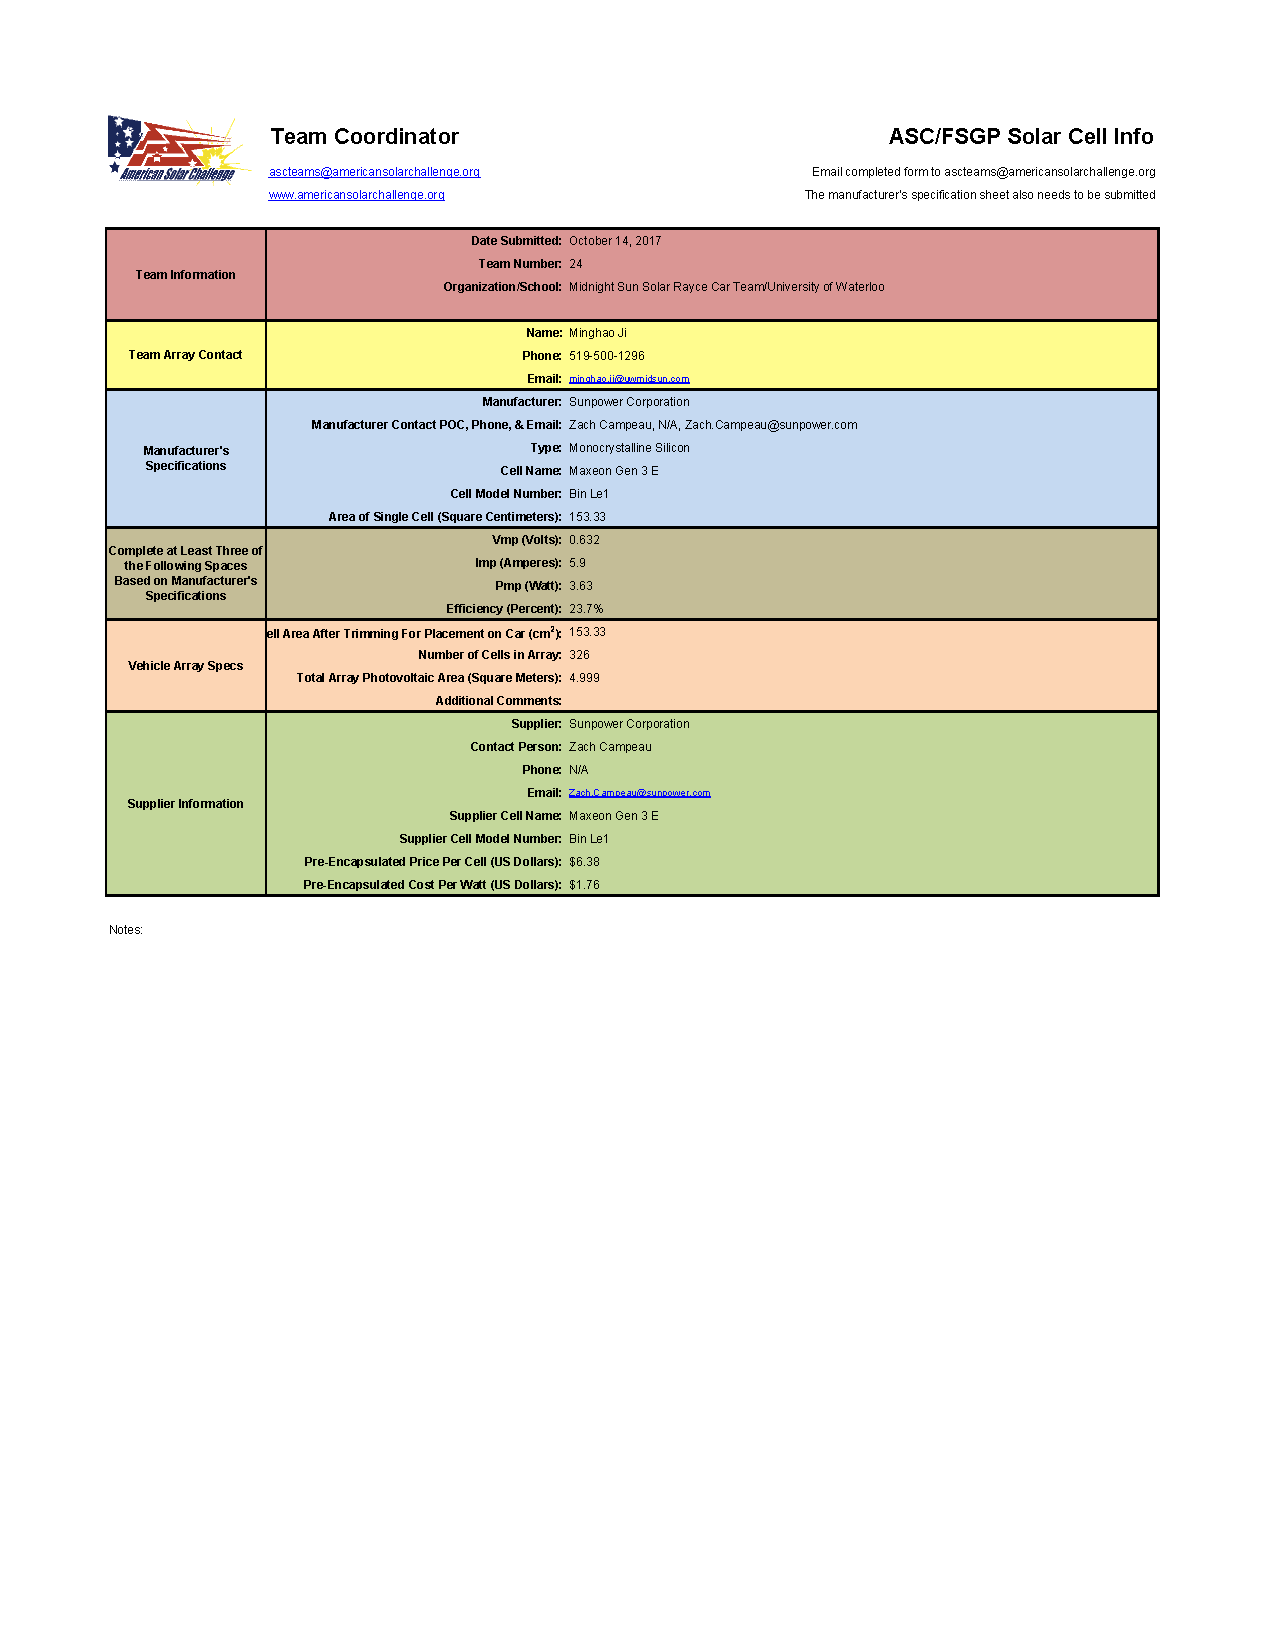
\includepdf[pages={-}]{forms/solar_cell_approval_form.pdf}

% Title Page
\begin{titlepage}
\large
\vspace*{2cm}
\centering

\includegraphics[width=.25\textwidth]{./figures/midnightSunLogoCircle.png} \\
\vspace{1.5cm}
{\LARGE \theteamname} \\
\theuniversityname \\
\vspace{2.2cm}
{\LARGE MSXII} \\
\vspace{0.4cm}
{\huge\bfseries \thetitle} \\
\vspace{0.2cm}
{\LARGE \thesubtitle} \\
\vspace{2.2cm}
\ifdefined \theauthor
\par Prepared by: \\
\theauthor \\
\theauthorcontact \\
\fi
\thedate \\
\vfill
\theteamwebsite \\
\theteamphone
\end{titlepage}

% Main Matter
\tableofcontents
\listoffigures % <-------------- uncomment for list of figures
%\listoftables % <-------------- uncomment for list of tables

\section{History}
Midnight Sun was founded in 1988 at the University of Waterloo. The team has produced 11 solar-powered vehicles since its inception, numbered MSI through MSXI. MSX and its predecessors have been traditional Challenger class cars. MSXI was the team's first attempt at a Cruiser class vehicle, which ultimately suffered from design issues relating to its monocoque design. With MSXII, the team has regrouped and designed a new Cruiser vehicle from the gound up, focussing strongly on reliability, safety, and manufacturability.

\section{Contacts}
Questions regarding the electrical design and implementation of MSXII should be directed to one of the following contacts:

\begin{table}[!h]
\centering
\begin{tabular}{llll}
\toprule
Name            & Title               & Phone        & Email \\
\midrule
Tak Alguire     & Project Manager     & 519-574-4610 & tak.alguire@uwmidsun.com \\
Minghao Ji      & Engineering Manager & 519-500-1292 & minghao.ji@uwmidsun.com \\
Titus Chow      & Electrical Lead     & 226-978-7104 & titus.chow@uwmidsun.com \\
\bottomrule
\end{tabular}
\end{table}

\section{Overview}
Midnight Sun XII's electrical system consists of high- and low-voltage domains that are electrically isolated for safety. The high-voltage system includes the Sunpower E-series solar cells, Nomura maximum power point trackers, Tritium motor controllers and NGM SCM-150 motors. These are externally-sourced components purchased by the team and interface with the vehicle's custom embedded systems.

The low-voltage system is comprised of custom circuit-boards serving several functions for monitoring and controlling the vehicle, primarily: driver controls, power distribution, battery management, and external lights. Several smaller PCBs are located throughout the vehicle to support various sensor interfacing and data collection functions. Most boards communicate over a unified CAN bus, with some nodes supporting smaller subsystems over I2C or SPI. The low-voltage power rail is normally provided by the main battery pack via DC-DC converters, but can also be switched to an auxiliary \SI{12}{\volt} Ni-MH battery during startup or fault modes.

Due to the different CAN specifications of the Tritium WaveSculptor motor controllers, they are allocated a separate powertrain CAN network which interfaces with the primary CAN bus via dedicated transceiver boards. A block diagram of all electrical systems is shown in Figure \ref{fig:msxii-electrical-full-block-diagram}. A block diagram of only the vehicle's high-voltage systems is shown in Figure \ref{fig:msxii-electrical-hv-block-diagram}.

\begin{figure}
\centering
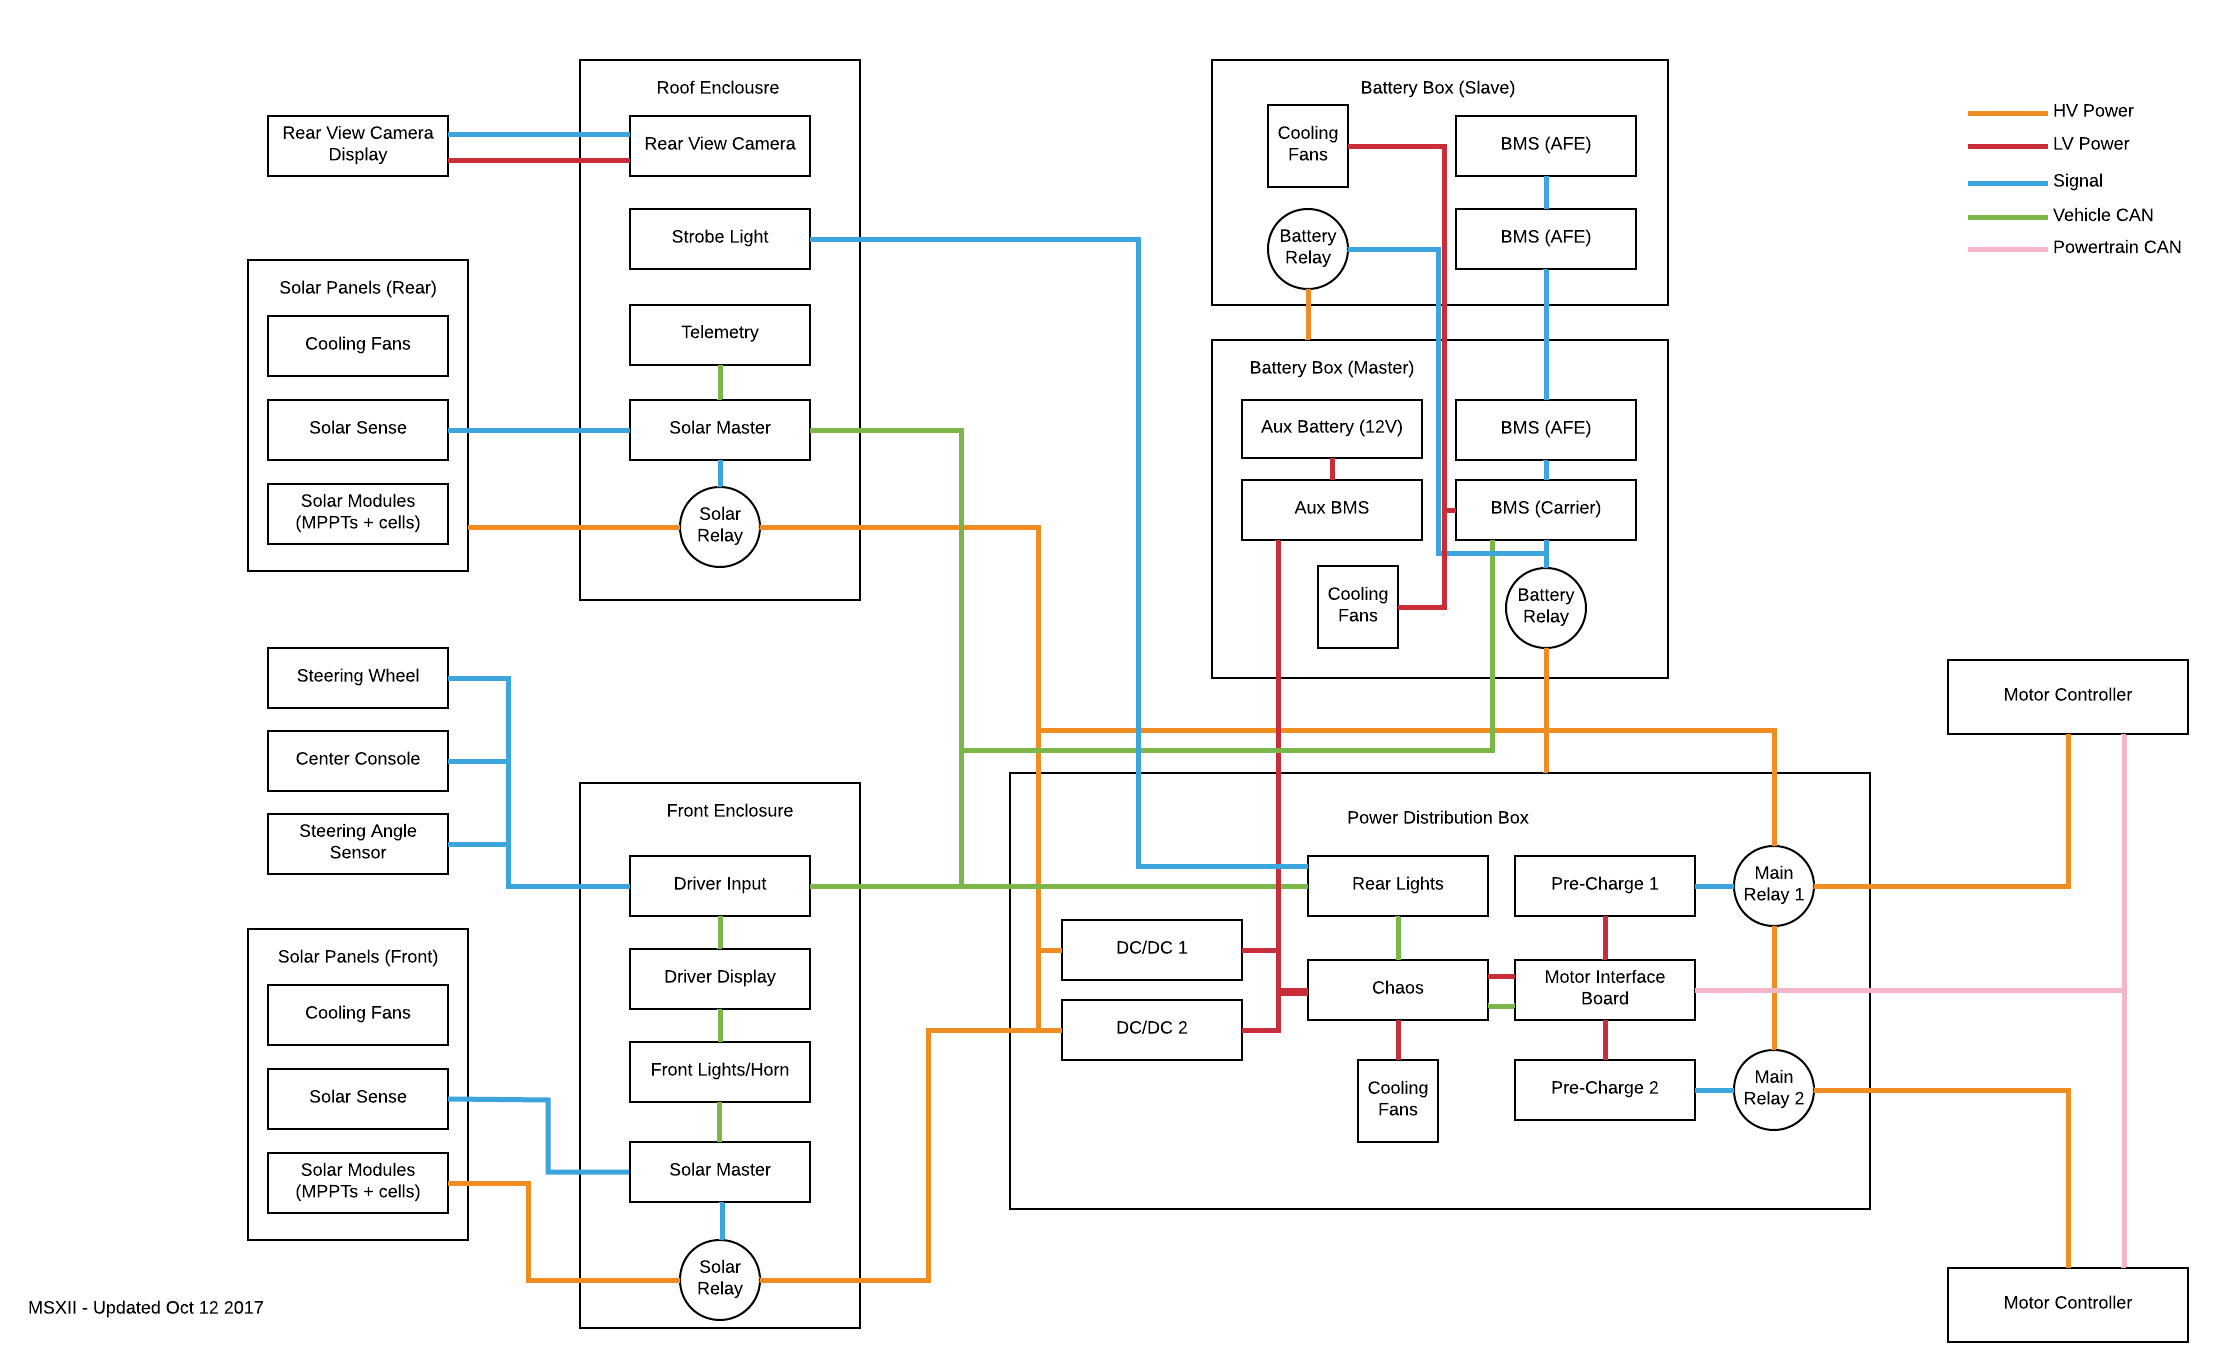
\includegraphics[width=\textwidth]{figures/msxii-electrical-full-block-diagram}
\caption{Block diagram of all electrical systems}
\label{fig:msxii-electrical-full-block-diagram}
\end{figure}

\begin{figure}
\centering
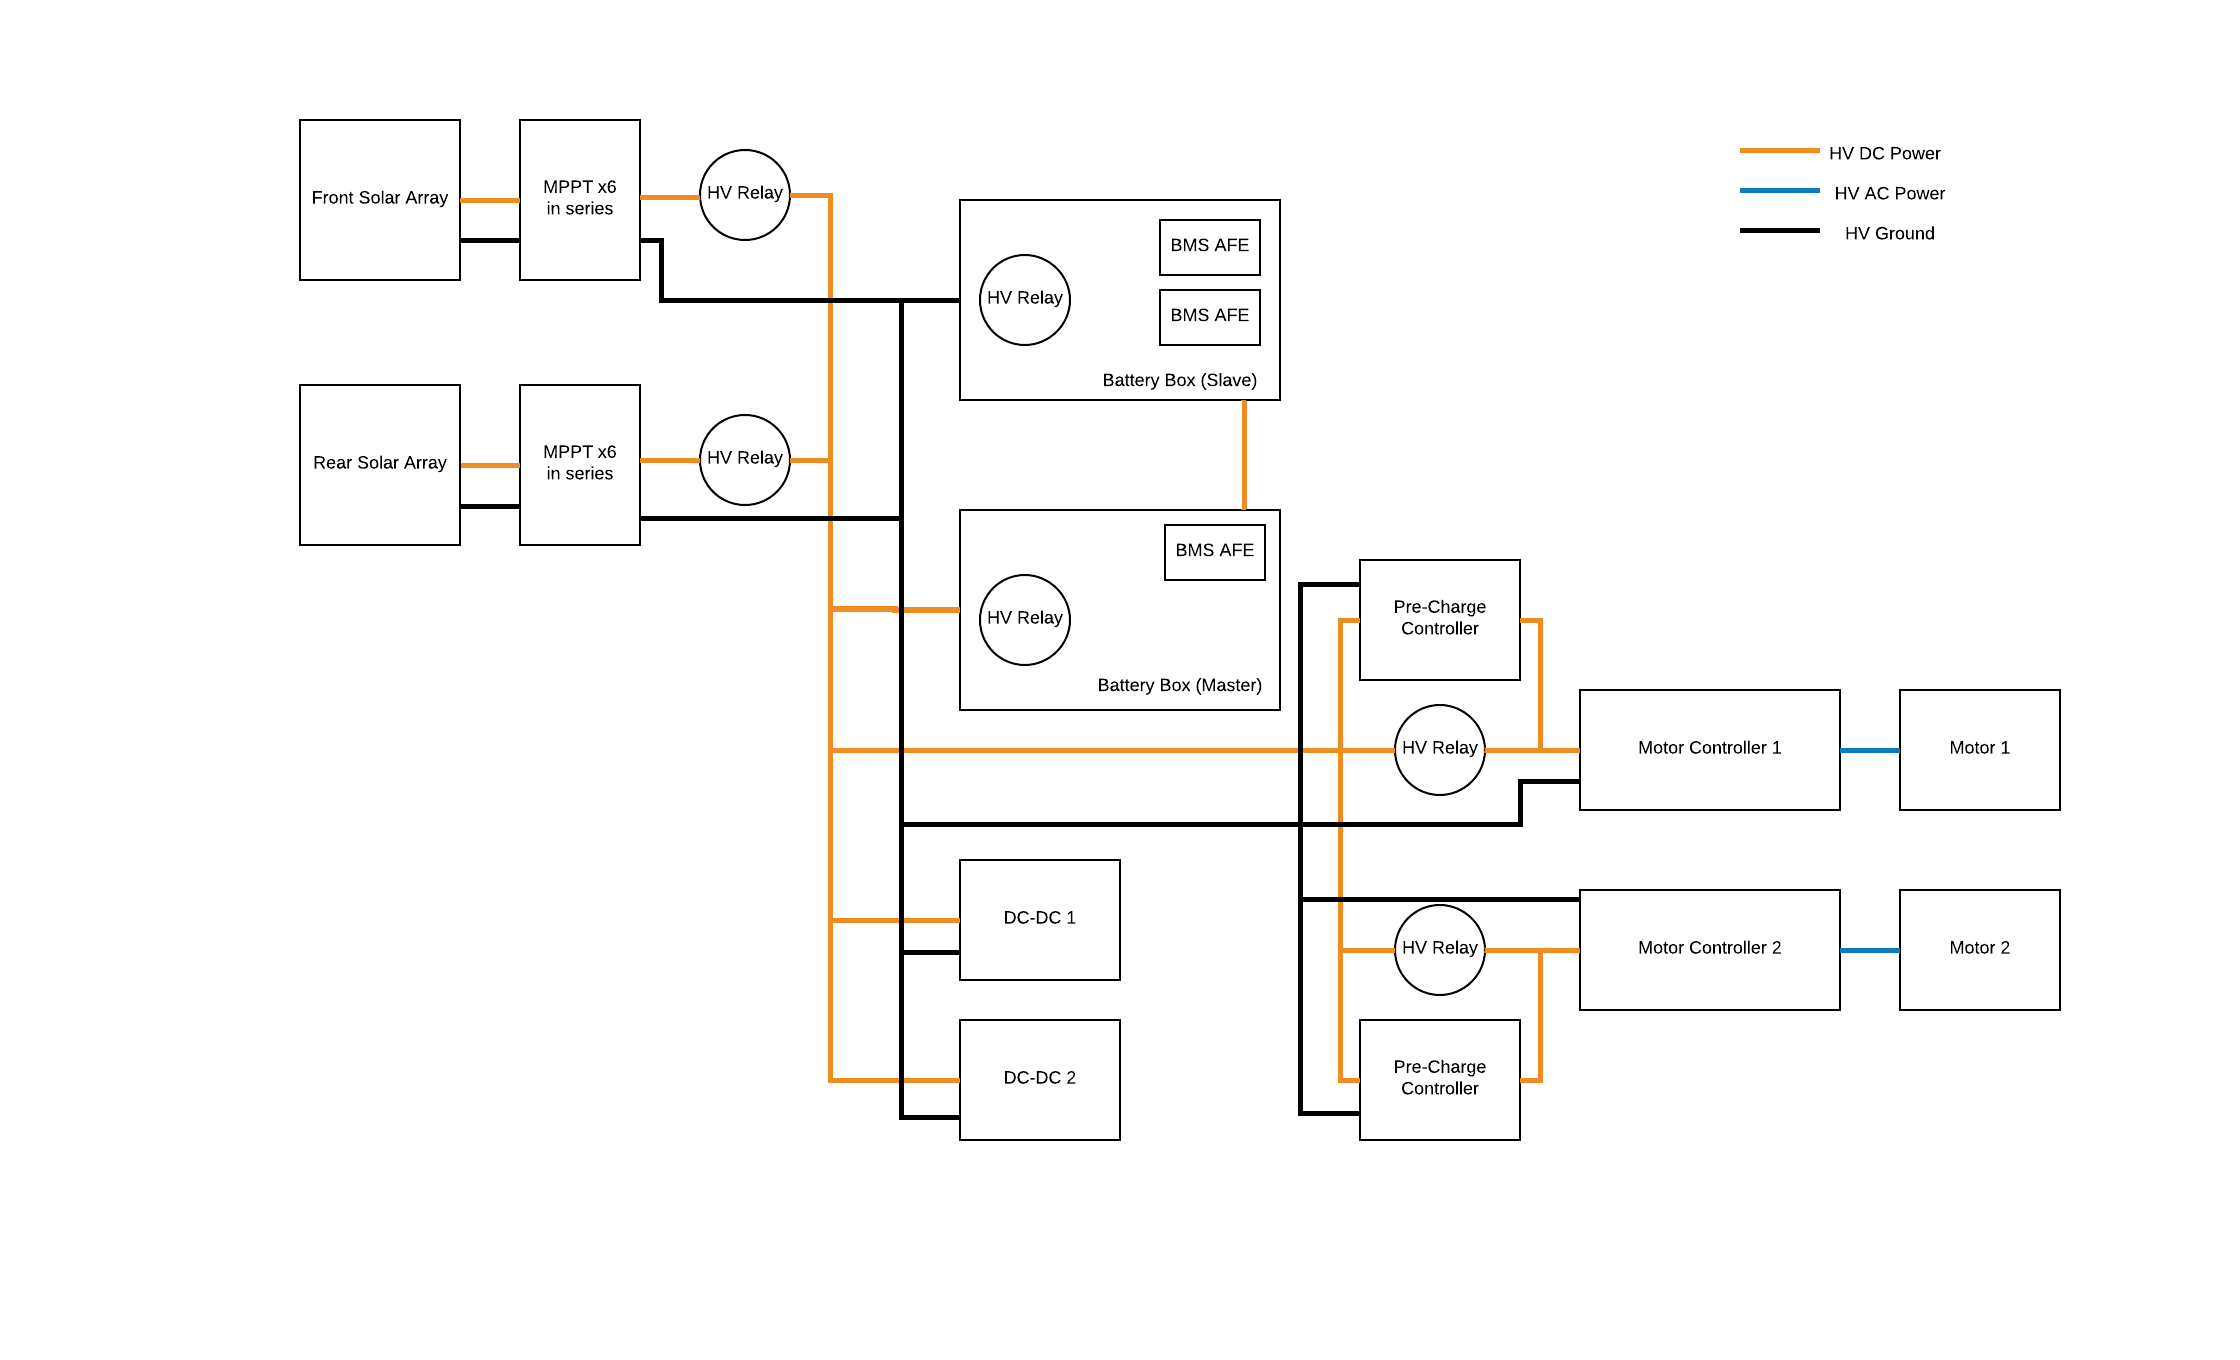
\includegraphics[width=\textwidth]{figures/msxii-electrical-hv-block-diagram}
\caption{Block diagram of all high-voltage electrical systems}
\label{fig:msxii-electrical-hv-block-diagram}
\end{figure}

\section{Battery}
For MSXII the team chose to use MJ1 18650 cells produced by LG Chem Ltd. 36 MJ1 cells are put in parallel to form a module, and 36 modules are put in series to provide a \SI{130.86}{\volt} nominal, \SI{16.5}{\kilo\watt\hour} capacity battery pack. Within each module, cells will be spot welded to nickel tabs, which are themselves soldered to copper bus bars forming a high-ampacity interconnect. Bus bars of adjacent modules are mechanically connected together to create series connections through the pack.

The cells were sourced from Liion Wholesale in early 2017.

\section{Testing Methodology}
Battery testing is expected to be completed in 4 main phases, outlined below.

\subsection{Phase One}
The first phase requires verification of the battery management system (BMS). This will test the system's ability to measure and monitor voltage, current, and temperature measurements from each of the modules. The system must be able to correctly respond to under-voltage, over-voltage, over-current, and over-temperature conditions to demonstrate that the BMS can actively protect the battery. Phase one is currently underway and is expected to be complete by November 2017. 

\subsection{Phase Two}
The second phase requires testing module performance and reliability. A prototype module containing 36 cells in parallel will be built and tested. This module will undergo charge cycle tests using a benchtop power supply and an electronic load. The BMS will be connected to log data and ensure safety. The team will then build 3 battery modules to test the series connections between modules. Phase two is expected to be complete by December 2017. 

\subsection{Phase Three}
The third phase involves the full manufacturing and testing of the battery pack. The team will be able to assess the overall performance of the battery and make necessary modifications to the cooling system prior to installing the battery in the car. The pack will be discharged at 1C, which is approximately \SI{120}{\ampere} of current. This will be accomplished by either powering the vehicle motors mounted to a dynamometer, or by using a salt water load with a resistance designed for the target current draw. Phase three is expected to be completed by the end of January 2018.

\subsection{Phase Four}
The final phase of battery testing will involve building a mechanical enclosure and integrating the pack into the vehicle. With a drivable vehicle, the team will be able to test the pack under real world conditions, and make any changes necessary prior to the race. Reliability of the modules and connections under harsh environmental conditions can be evaluated during road tests. Since this requires the vehicle to be in a drivable state, it is expected to begin in April or May 2018 and finish before July. 

% Bibliography
%\pagebreak
%\printbibliography

% Appendix
\pagebreak
\appendix

\end{document}
